\section{Query}\label{sec:query}

\subsection{¿Qué es la query?}
\begin{frame}{¿Qué es la query?}
        La query es el texto que el usuario quiere buscar dentro de los documentos.\\
        \pause  \vspace*{0.3cm}     
        Para la búsqueda realizada por un usuario (query) se dispone de una clase TextPrcessor,
        la cual calculara un score por cada documento, donde ese score es la similitud que
        posee la query con un documento determinado.\\
        \pause \vspace*{0.3cm}
        Este score se calcula a traves de la similitud coseno
\end{frame}

\subsection{Similitud Coseno}
\begin{frame}{¿Qué es la similitud coseno?}
        \begin{center}
                La similitud coseno es una medida de la similitud existente entre dos vectores en un espacio 
                que posee un producto interior con el que se evalúa el valor del coseno del ángulo comprendido 
                entre ellos.
        \end{center}
\end{frame}

\begin{frame}{Intervalo de la similitud coseno}
        Esta función trigonométrica proporciona un valor igual a 1 si el ángulo comprendido es cero,
        es decir si ambos vectores apuntan a un mismo lugar. \pause
        Cualquier ángulo existente entre los vectores, el coseno arrojaría un valor inferior a uno. \pause
        Si los vectores fuesen ortogonales el coseno se anularía, \pause
        y si apuntasen en sentido contrario su valor sería -1. \\
        \pause \vspace*{0.3cm}
        De esta forma, el valor de esta métrica se encuentra entre -1 y 1, es decir en el intervalo cerrado [-1,1].
\end{frame}

\begin{frame}{Calculo de la similitud coseno}
        Primero se tratará a la query como un documento más, se calculará su TF y se guardará
        en un vector, que en terminos de programacion, es una matriz, de una fila o una colummna.\\
        \pause \vspace*{0.3cm}
        Luego se multiplicará la matriz de TF-IDF con el vector de la query, es decir: \\
        \begin{equation}\nonumber
                \sum_{k = 0}^{p} M_{ik} \cdot V_{kp}
        \end{equation}
        donde: $M_{ik}$, $V_{kp}$, i, p representan respectivamente a un elemento de la matriz, 
        un elemento del vector, las filas y las columnas.\\
        \pause \vspace*{0.3cm}
        Estos valores se guardan en un array o vector, llamado como, \textit{vectorResultante} 
\end{frame}

\begin{frame}{Calculo de la similitud coseno}
        Además se obtiene la norma de la matriz de TF-IDF como la del vector. \\
        \pause \vspace*{0.3cm}
        La norma de una matriz fila puede calcularse como:
        \begin{equation}\nonumber
                \sqrt{\sum_{k = 0}^{p} a_k}
        \end{equation}       
        donde: p son las columnas y $a_k$ un elemento de la matriz fila. \\
        \pause \vspace*{0.3cm}
        Por tanto, al final se obtendrán un vector (matriz columna) por parte de la matriz 
        y un numero por parte del vector.
\end{frame}

\begin{frame}{Calculo de la similitud coseno}
        Por ultimo, para calcular la similitud coseno se divide cada elemento del \textit{vectorResultante} ($V_i$)
        entre la multiplicación de la norma de la query ($NQ$) por el correspondiente elemento de la norma de la matriz ($N_i$).\\

        \begin{equation}\nonumber
                \frac{V_i}{NQ \cdot N_i}
        \end{equation}
\end{frame}

\subsection{Operadores}
\begin{frame}{Operadores}
        Un operador es un caracter que cuando aparece en la query, en vez de ser tratado como texto plano,
        modifica el comportamiento de cómo se realiza la busqueda. Por ejemplo:
        \begin{itemize}
                \item El operador “ * ”: aumenta la importancia que tiene una palabra en la búsqueda.
                \item El operador “ ! ”: indica que la palabra a la que modifica no debe aparecer en los resultados de
                la búsqueda. 
                \item El operador “ \textasciicircum \space ": indica que la palabra a la que modifica siempre debe aparecer en los resultados
                de la búsqueda.
                \item El operador “ \textasciitilde \space ”: indica que las dos palabras a sus extremos deben aparecen los más cercanos
                posibles en los resultados de la búsqueda.   
        \end{itemize}
\end{frame}

\subsection{Ejemplos de resultados de busqueda}
\begin{frame}{Ejemplos de resultados de busqueda}
        \begin{figure}
                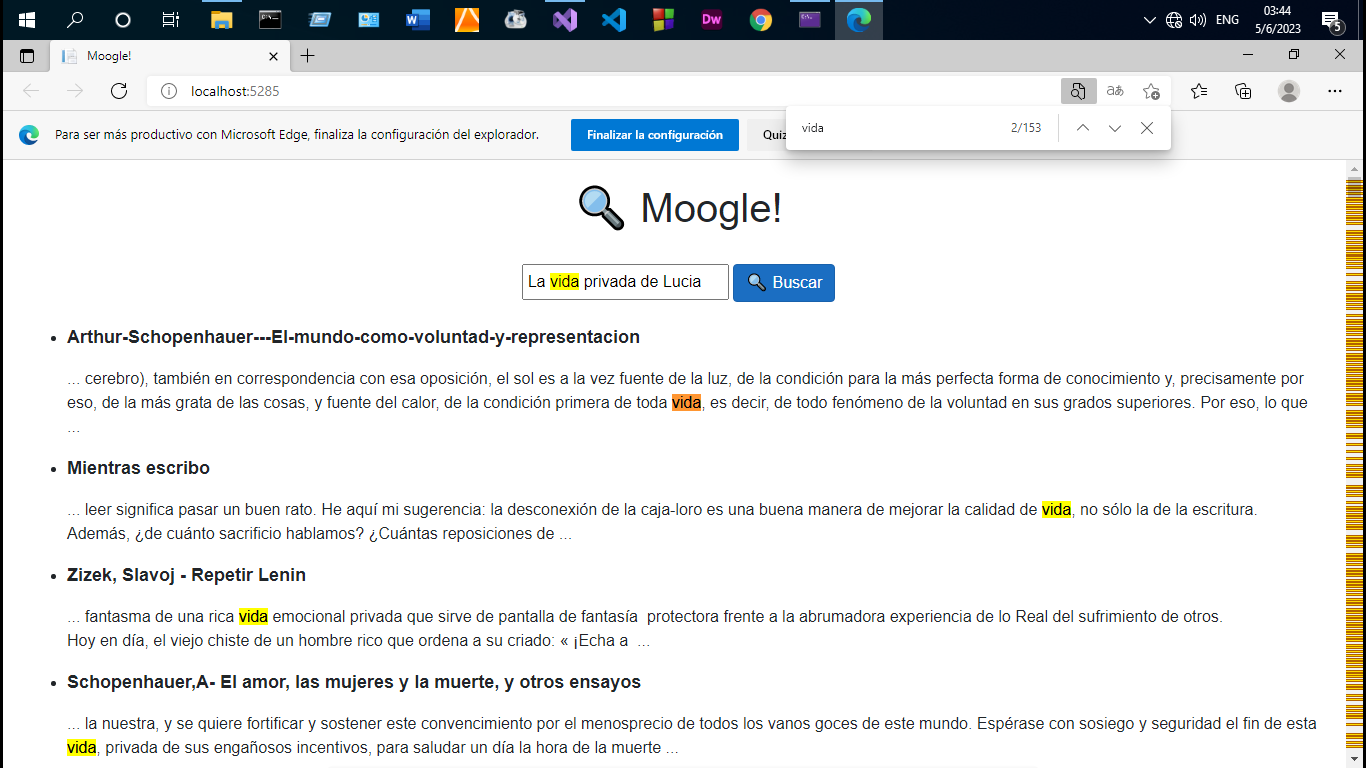
\includegraphics[width=0.9\framewidth]{../Informe/fotos/08 - Resultados (1).png}
        \end{figure}
\end{frame}

\begin{frame}{Ejemplos de resultados de busqueda}
        \begin{figure}
                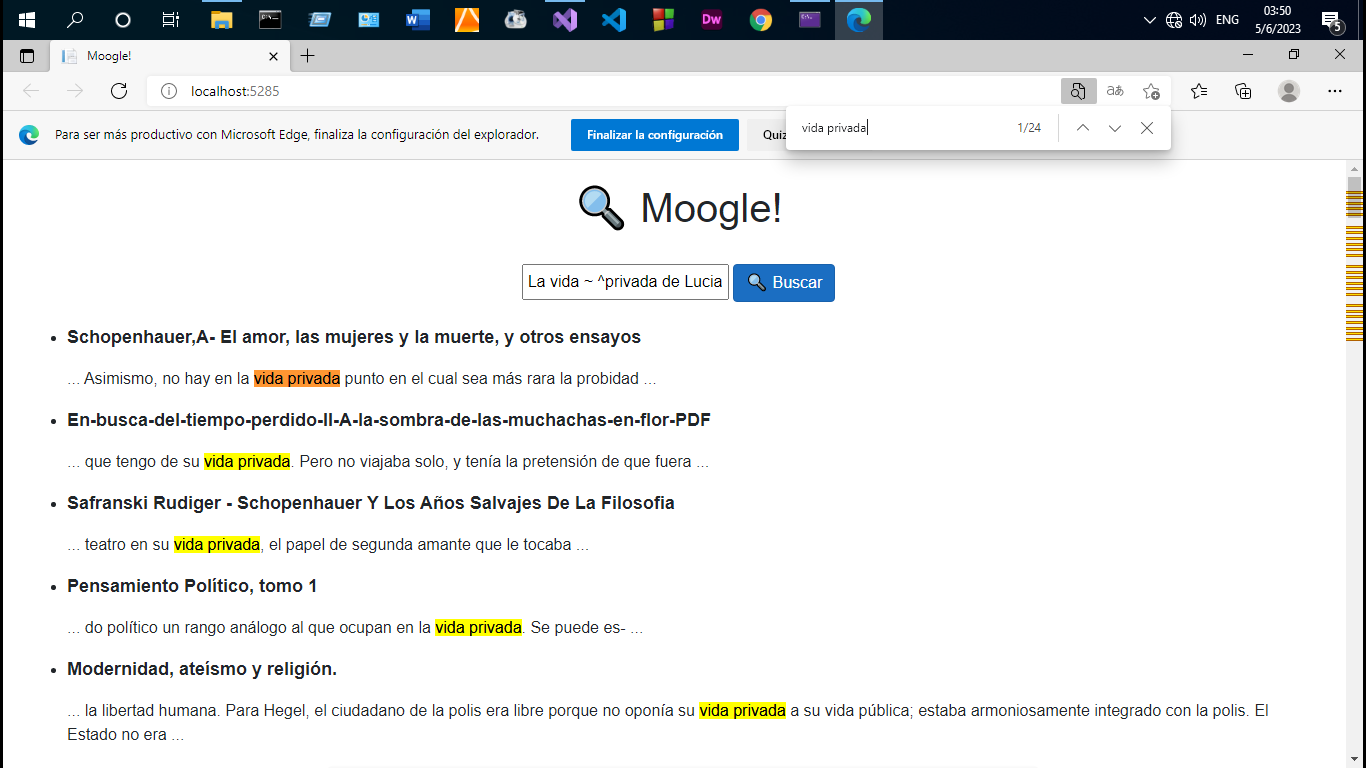
\includegraphics[width=0.9\framewidth]{../Informe/fotos/13 - Resultados (6).png}
        \end{figure}
\end{frame}

\begin{frame}{Ejemplos de resultados de busqueda}
        \begin{figure}
                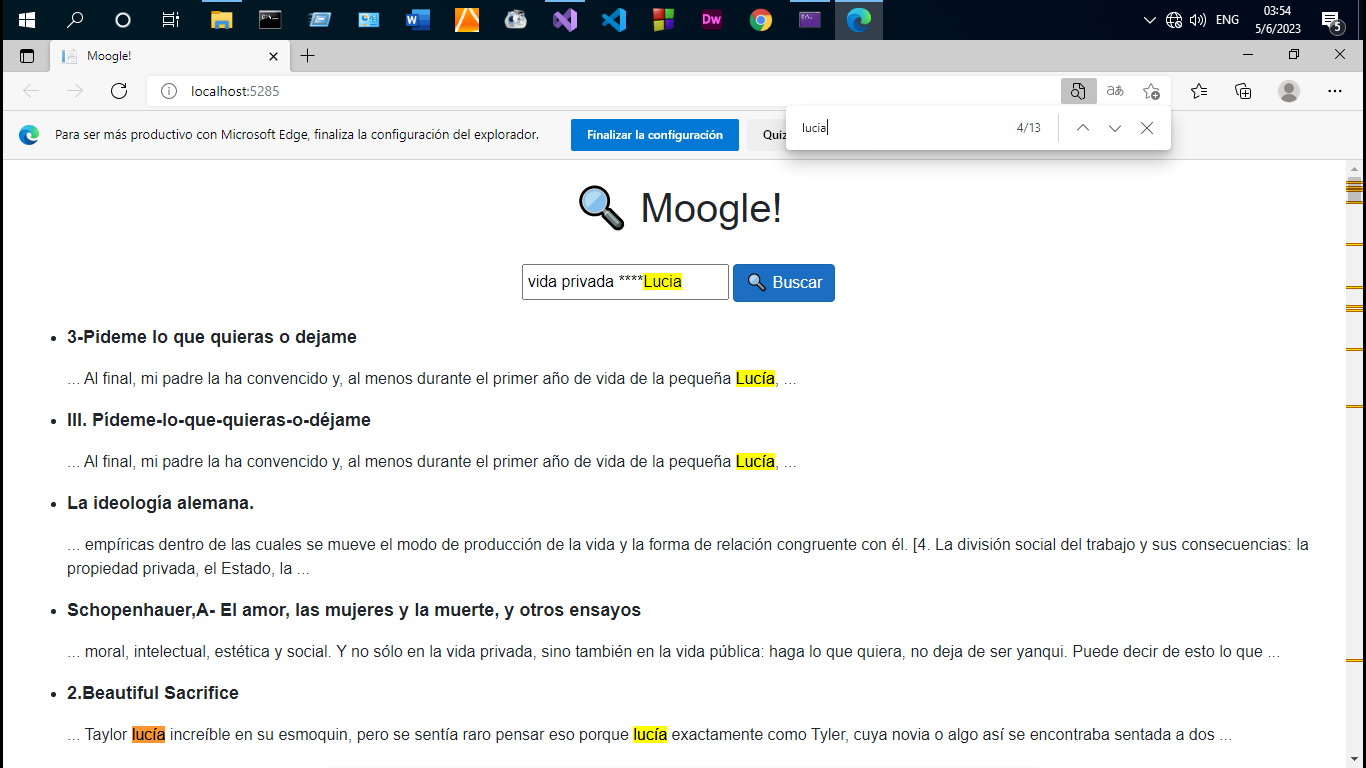
\includegraphics[width=0.9\framewidth]{../Informe/fotos/14 - Resultados (7).png}
        \end{figure}
\end{frame}